% Copyright (C) 2014-2020 by Thomas Auzinger <thomas@auzinger.name>

\documentclass[draft,final]{vutinfth} % Remove option 'final' to obtain debug information.

% Load packages to allow in- and output of non-ASCII characters.
\usepackage{lmodern}        % Use an extension of the original Computer Modern font to minimize the use of bitmapped letters.
\usepackage[T1]{fontenc}    % Determines font encoding of the output. Font packages have to be included before this line.
\usepackage[utf8]{inputenc} % Determines encoding of the input. All input files have to use UTF8 encoding.

% Extended LaTeX functionality is enables by including packages with \usepackage{...}.
\usepackage{amsmath}    % Extended typesetting of mathematical expression.
\usepackage{amssymb}    % Provides a multitude of mathematical symbols.
\usepackage{mathtools}  % Further extensions of mathematical typesetting.
\usepackage{microtype}  % Small-scale typographic enhancements.
\usepackage[inline]{enumitem} % User control over the layout of lists (itemize, enumerate, description).
\usepackage{multirow}   % Allows table elements to span several rows.
\usepackage{booktabs}   % Improves the typesettings of tables.
\usepackage{subcaption} % Allows the use of subfigures and enables their referencing.
\usepackage[ruled,linesnumbered,algochapter]{algorithm2e} % Enables the writing of pseudo code.
\usepackage[usenames,dvipsnames,table]{xcolor} % Allows the definition and use of colors. This package has to be included before tikz.
\usepackage{nag}       % Issues warnings when best practices in writing LaTeX documents are violated.
\usepackage{todonotes} % Provides tooltip-like todo notes.

% added by me
\usepackage{listings}
\usepackage{color}
\usepackage{wrapfig}

\usepackage{hyperref}  % Enables cross linking in the electronic document version. This package has to be included second to last.
\usepackage[acronym,toc]{glossaries} % Enables the generation of glossaries and lists fo acronyms. This package has to be included last.

% added by me: https://www.overleaf.com/learn/latex/LaTeX_Graphics_using_TikZ%3A_A_Tutorial_for_Beginners_(Part_3)%E2%80%94Creating_Flowcharts
\usepackage{tikz}
\usetikzlibrary{shapes.geometric, arrows, fit}

\tikzstyle{startstop} = [rectangle, rounded corners,
minimum width=3cm,
minimum height=1cm,
text centered,
draw=black,
fill=red!30]

\tikzstyle{io} = [trapezium,
trapezium stretches=true,
trapezium left angle=70,
trapezium right angle=110,
minimum width=3cm,
minimum height=1cm, text centered,
draw=black, fill=blue!30]

\tikzstyle{process} = [rectangle,
minimum width=3cm,
minimum height=1cm,
text centered,
text width=3cm,
draw=black,
fill=orange!30]

\tikzstyle{decision} = [diamond,
minimum width=3cm,
minimum height=1cm,
text centered,
draw=black,
fill=green!30]
\tikzstyle{arrow} = [thick,->,>=stealth]

\tikzstyle{inst} = [rectangle, rounded corners,
minimum width=3cm,
minimum height=1cm,
text centered,
text width=3cm,
draw=black,
fill=blue!30]

% added by me
\lstset{language=C++}
%\definecolor{basicStyleColor}{RGB}{0,0,90}
\definecolor{basicStyleColor}{RGB}{0,0,150}
\lstset{
    language=C++,
    breaklines=true,
%    breakatwhitespace=true,
    basicstyle=\ttfamily\color{basicStyleColor},
}

% Define convenience functions to use the author name and the thesis title in the PDF document properties.
\newcommand{\authorname}{Robert Obkircher} % The author name without titles.
\newcommand{\thesistitle}{On-Stack Replacement in the CACAO VM} % The title of the thesis. The English version should be used, if it exists.

% Set PDF document properties
\hypersetup{
    pdfpagelayout   = TwoPageRight,           % How the document is shown in PDF viewers (optional).
    linkbordercolor = {Melon},                % The color of the borders of boxes around crosslinks (optional).
    pdfauthor       = {\authorname},          % The author's name in the document properties (optional).
    pdftitle        = {\thesistitle},         % The document's title in the document properties (optional).
    pdfsubject      = {Subject},              % The document's subject in the document properties (optional).
    pdfkeywords     = {a, list, of, keywords} % The document's keywords in the document properties (optional).
}

\setpnumwidth{2.5em}        % Avoid overfull hboxes in the table of contents (see memoir manual).
\setsecnumdepth{subsection} % Enumerate subsections.

\nonzeroparskip             % Create space between paragraphs (optional).
\setlength{\parindent}{0pt} % Remove paragraph identation (optional).

\makeindex      % Use an optional index.
\makeglossaries % Use an optional glossary.
%\glstocfalse   % Remove the glossaries from the table of contents.

% Set persons with 4 arguments:
%  {title before name}{name}{title after name}{gender}
%  where both titles are optional (i.e. can be given as empty brackets {}).
\setauthor{}{\authorname}{}{male}
\setadvisor{Ao.Univ.Prof. Dipl.-Ing. Dr.techn.}{Andreas Krall}{}{male}

% For bachelor and master theses:
%\setfirstassistant{Pretitle}{Forename Surname}{Posttitle}{male}
%\setsecondassistant{Pretitle}{Forename Surname}{Posttitle}{male}
%\setthirdassistant{Pretitle}{Forename Surname}{Posttitle}{male}

% For dissertations:
%\setfirstreviewer{Pretitle}{Forename Surname}{Posttitle}{male}
%\setsecondreviewer{Pretitle}{Forename Surname}{Posttitle}{male}

% For dissertations at the PhD School and optionally for dissertations:
%\setsecondadvisor{Pretitle}{Forename Surname}{Posttitle}{male} % Comment to remove.

% Required data.
\setregnumber{11807844}
\setdate{01}{01}{2001} % Set date with 3 arguments: {day}{month}{year}.
\settitle{\thesistitle}{On-Stack Replacement in der CACAO VM} % Sets English and German version of the title (both can be English or German). If your title contains commas, enclose it with additional curvy brackets (i.e., {{your title}}) or define it as a macro as done with \thesistitle.
%\setsubtitle{Optional Subtitle of the Thesis}{Optionaler Untertitel der Arbeit} % Sets English and German version of the subtitle (both can be English or German).

% Select the thesis type: bachelor / master / doctor / phd-school.
% Bachelor:
\setthesis{bachelor}
%
% Master:
%\setthesis{master}
%\setmasterdegree{dipl.} % dipl. / rer.nat. / rer.soc.oec. / master
%
% Doctor:
%\setthesis{doctor}
%\setdoctordegree{rer.soc.oec.}% rer.nat. / techn. / rer.soc.oec.
%
% Doctor at the PhD School
%\setthesis{phd-school} % Deactivate non-English title pages (see below)

% For bachelor and master:
\setcurriculum{Software \& Information Engineering}{Software \& Information Engineering} % Sets the English and German name of the curriculum.

% For dissertations at the PhD School:
\setfirstreviewerdata{Affiliation, Country}
\setsecondreviewerdata{Affiliation, Country}


% My custom macros:


\begin{document}

    \frontmatter % Switches to roman numbering.
% The structure of the thesis has to conform to the guidelines at
%  https://informatics.tuwien.ac.at/study-services

    \addtitlepage{naustrian} % German title page (not for dissertations at the PhD School).
    \addtitlepage{english} % English title page.
    \addstatementpage

%    \begin{danksagung*}
%    \end{danksagung*}

%    \begin{acknowledgements*}
%    \end{acknowledgements*}

    \begin{kurzfassung}
        Beim On-Stack-Replacement geht es darum, dynamisch zwischen verschiedenen Maschinencode-Versionen einer Funktion zu wechseln.
        CACAO VM ist eine zu Forschungszwecken entwickelte Virtuelle Maschine für Java,
        die OSR für profilgesteuerte Optimierung einsetzt.
        Diese Arbeit verbessert die unvollständige Implementierung,
        um die zweite Compilerstufe besser zu nutzen
        und behebt mehrere andere Fehler.
        Die Auswertung erfolgt durch Erweiterung der existierenden Tests
        und mithilfe der SpecJVM2008-Benchmark-Suite.
        Letztere zeigt Leistungsverbesserungen,
        aber drei der Teilbenchmarks produzieren noch ungültige Ergebnisse.
    \end{kurzfassung}

    \begin{abstract}
        On-Stack Replacement (OSR) is a technique for dynamically switching between different machine-code versions of a specific function.
        CACAO VM is a research Java Virtual Machine that uses OSR for profile-guided optimizations.
        This work improves the incomplete implementation
        to make better use of the second-stage compiler
        and fixes multiple unrelated bugs.
        We evaluate the result by extending the existing test suite
        and by running the SpecJVM2008 benchmark suite.
        The latter shows improvements in performance,
        but three of the sub-benchmarks still produce invalid results.
    \end{abstract}

% Select the language of the thesis, e.g., english or naustrian.
    \selectlanguage{english}

% Add a table of contents (toc).
    \tableofcontents % Starred version, i.e., \tableofcontents*, removes the self-entry.

% Switch to arabic numbering and start the enumeration of chapters in the table of content.
    \mainmatter


    \chapter{Introduction}


    \section{The CACAO VM}

    CACAO is an open-source research Java Virtual Machine (JVM)
    that was developed at TU Wien.\cite{cacao-homepage,cacao-repo,cacao-64bit-jit}

    A JVM is an abstract computing machine that loads and executes class files.
    A class file is a binary format that describes the fields, methods, and other information of a class.
    The instructions are encoded in stack-based bytecode with a predetermined maximum operand stack size.
    They operate on primitive types (\emph{numeric}, \emph{boolean}, \emph{returnAddress}) and references (to \emph{class}, \emph{array}, and \emph{interface types}).
    Values can also be stored in an array of local variables,
    where \emph{long} and \emph{double} take up two consecutive slots.
    Method invocation pops the arguments from the operand stack,
    and creates a new frame, where they become the first local variables.
    The full specifications of the JVM and of the Java programming language, which is compiled to it, can be found online\cite{JavaSE}.

    Unlike other JVM implementations,
    CACAO relies on a compile-only approach, without a bytecode interpreter.
    Consequently, the just-in-time (JIT) compiler was optimized for compilation speed.
    When it compiles a method, it parses the bytecode into an array of instructions.
    Then it replaces the operand stack with variables during stack analysis,
    and it performs additional checks to verify the bytecode.
    Finally, it builds a control flow graph, allocates registers, and generates machine code.
    To improve performance for frequently executed code,
    various optional optimizations such as adaptive inlining were implemented,
    which led to a need for on-stack replacement\cite{10.1145/1294325.1294356}.

    After CACAO had been ported from C to C++, a second-stage compiler\cite{EislJosef2013Offt} was added
    with the main goal of making it possible to easily add new optimizations.
    It uses a much more flexible graph-based intermediate representation (IR)
    and it increased the complexity of on-stack replacement.

    From now on, we will refer to the original compiler as the \emph{baseline compiler} and
    to the optimizing compiler as \emph{compiler2}.
    We use \emph{source state} and \emph{execution state} to distinguish between
    the state of the virtual and physical machine.


    \section{On-Stack Replacement}

    \begin{figure}[h]
        \begin{lstlisting}
        int count() {
            int i = 0;
            while(i < 1000000) i += 1;
            return i;
        }
        \end{lstlisting}
        \caption{A naive translation may put \lstinline{i} in a register or on the stack, while an optimized one will not even do the loop.}
    \end{figure}

    On-stack replacement (OSR) refers to the replacement of executing machine code with another version.
    This is usually accomplished by first pausing the thread at a convenient location.
    Then the new code is looked up or generated.
    Unless it was tailored to this location, the replacement mechanism may also need to adjust the stack and registers.
    Finally, execution can resume at the new program counter.

    The technique was initially developed for modifying and debugging optimized programs\cite{10.1145/191081.191116},
    but it was later adopted by just-in-time (JIT) compilers to improve performance.
    It enables quick start up times and excellent steady-state performance
    because expensive optimizations can selectively be applied to frequently executed code.
    The profiling information that is required to decide which code should be recompiled
    is usually collected with counters in the unoptimized code.
    It can then also be used for profile-guided optimization to specialize code to the actual workload of the program.
    Optimization is typically triggered when a counter reaches a certain threshold.
    Recompilations may also be triggered for adaptive optimization
    when the execution profile changes
    or if speculative optimizations were performed based on transient program facts.
    Optimized code may also use deoptimization for rare paths such as throwing exceptions.

    The locations where OSR can be performed are usually limited to specific points
    to simplify the transition, to limit amount of meta-information, and to allow for values to be optimized away.
    In CACAO these locations are called \emph{replacement points}
    and the meta-information describes where values
    from the source state are located in the native stack frame or registers.
    During replacement, the allocation information of the two corresponding replacement points
    in both versions of the code is used to rewrite the execution state.
    This is more flexible than generating custom code for the transition
    because the target code is not tied to the source.

    A replacement point that was created by the baseline compiler can be used for both
    transitioning into and out of the code.
    This is possible because the code essentially uses the same set of values as the virtual machine.
    In compiler2, this is not the case.
    To make it possible to transition away from the code, a special instruction takes all required values as operands to ensure that they are actually computed.
    The other direction essentially requires a special entrypoint that reads the source state.


    \section{Motivation}

    The current OSR mechanism in CACAO is incomplete and contains bugs.
    There are two test cases that likely fail because of invalid deoptimization.
    Furthermore, the inlining implementation\cite{MethodInlining} that was recently added to compiler2 is not yet compatible with OSR.
    Using countdown traps to switch from unoptimized to optimized code is also severely limited.
    It is only possible at method entry, where the stack doesn't need to be modified,
    but long-running loops aren't yet optimized.


    \section{Aim of the Work}

    The goal of this work is to improve the OSR mechanisms of CACAO.
    Deoptimization should work more reliably and support inlining,
    and it should also become possible to switch from unoptimized code to optimized code within loops.
    Correctness and performance will be evaluated with tests and benchmarks.


    \chapter{Related Work}


    \section{CACAO}

    \textit{Adaptive Inlining and On-Stack Replacement in the CACAO Virtual Machine}\cite{10.1145/1294325.1294356}
    describes the implementation of inlining and on-stack replacement in the baseline compiler.

    Compiler2 was introduced in \textit{Optimization Framework for the CACAO VM}\cite{EislJosef2013Offt}.
    The thesis describes how the two intermediate representations are transformed by a pipeline of passes.

    \textit{Method Inlining in the Second Stage Compiler of the CACAO VM}\cite{MethodInlining} describes the recently added implementation of inlining for compiler2.


    \section{On-Stack Replacement}


    \textit{A Survey of Adaptive Optimization in Virtual Machines}\cite{AdapOptSurvey} surveys adaptive optimization technology in virtual machines.

    The paper \textit{On-Stack Replacement, Distilled}\cite{10.1145/3192366.3192396} presents a provably correct OSR framework,
    and evaluates an implementation in LLVM.

    The document \textit{OSR in the CLR}\cite{CLR-OSR} in the .NET Runtime repository describes various design considerations that
    went into a fully functioning prototype implementation of OSR for the CLR.
    It focuses on the transition from unoptimized to optimized code, because their optimizing
    compiler doesn't do speculative optimization and thus doesn't require deoptimization.
    They discuss the requirements of an OSR implementation,
    how and where transitions can be implemented,
    how they can be triggered by counters,
    and whether optimized code should have one or multiple entrypoints.
    Most of the points in the section about complications aren't relevant,
    because the JVM doesn't have features such as references to local variables.


    \chapter{Background}

    This chapter gives an overview of the initial state of OSR in CACAO.
    Some details are specific to the \texttt{x86\_64} architecture.


    \section{Existing OSR Implementation}

    \begin{figure}
        \centering
        \begin{tikzpicture}[node distance=3cm]
            \node (stub) [startstop] {Stub Code};
            \node (h) [decision, below of=stub, align=center] {compiler2\\possible};
            \node (bl2) [process, right of=h, xshift=2cm] {Baseline Code\\with Counters};
            \node (c2success) [decision, right of=bl2, xshift=2cm, align=center] {compiler2\\success};
            \node (c2) [process, below of=c2success] {Compiler2 Code};
            \node (bl) [startstop, below of=bl2, xshift=-1.5cm] {Baseline Code};

            \draw [arrow] (stub) -- node[anchor=west]{jit\_compile} (h);
            \draw [arrow] (h) -- node[anchor=west]{no} (bl);
            \draw [arrow] (h) -- node[anchor=north]{yes} (bl2);
            \draw [arrow] (bl2) -- node[align=center]{after 100k\\times} (c2success);
            \draw [arrow] (c2success) -- node[anchor=west]{yes} (c2);
            \draw [arrow] (c2success) -- node[anchor=south]{no} (bl);
            \draw [arrow] (c2) -- node[anchor=south]{deoptimize} (bl);
        \end{tikzpicture}
        \caption{Versions of Machine Code for a Function}
        \label{fig:code-versions}
    \end{figure}

    The original baseline compiler already supported OSR with multiple optimization levels,
    but since compiler2 was introduced,
    this has been disabled,
    and the baseline compiler has only been used in two modes:
    one where it produces normal code,
    and another one where it also emits countdown traps.
    Figure\ref{fig:code-versions} visualizes the different machine code versions for a function.
    Initially, a stub lazily triggers compilation upon the first invocation,
    where a heuristic determines whether instrumented code should be produced.
    Compiler2 is called eventually,
    if counters are hit often enough.
    However, in the initial state only a single countdown trap was placed before the method prolog,
    because in that case OSR is almost trivial,
    as no stack or register modifications are required.
    There was no OSR of long-running loops.
    When compiler2 makes an assumption or can't compile an instruction, it emits a deoptimization instruction.
    Due to the heuristic this rarely happens outside of test cases.


    \section{Replacement Points}

    A replacement point is represented by the following struct:
    \begin{lstlisting}
struct rplpoint {
    u1 *pc;
    methodinfo *method;
    rplpoint *parent;
    rplalloc *regalloc;
    s4 id;
    s4 callsize;
    unsigned int regalloccount:20;
    Type type:4;
    unsigned int flags:8;
    u1 *patch_target_addr;
};
    \end{lstlisting}
    The program counter \lstinline{pc} can be used to look up the machine code that a replacement point belongs to.
    Within that code, it is identified by the \lstinline{method} and the instruction \lstinline{id}.
    The mapping between source and execution state is given by \lstinline{regalloc} and \lstinline{regalloccount}.
    The \lstinline{parent} would be required for inlining, but it was unused just like the \lstinline{type}.
    The flags indicate whether the replacement point is trappable, has a countdown, is a deoptimization point, and whether it has an active trap.
    When patching the caller, the return address is used to look up the replacement point before the invoke instruction
    to get its \lstinline{callsize} and \lstinline{patch_target_addr}.

    During code generation, the baseline compiler places replacement points and countdown traps.
    However, there was a bug which meant that not all replacement points were initialized correctly.


    \section{It's a Trap!}

    CACAO uses signal handlers to implement certain exceptions and to trigger the compiler.
    On \texttt{x86\_64} they are registered for \lstinline{SIGSEGV}, \lstinline{SIGILL}, and \lstinline{SIGFPE}.
    They call the platform-independent function \lstinline{void trap_handle(int sig, void *xpc, void *context)},
    which in turn uses a machine-dependent function \lstinline{md_executionstate_read} to
    copy registers from the OS context into a \lstinline{struct executionstate_t}.

    Traps are implemented via a mov instruction that reads from the first page in memory,
    which is marked \lstinline{PROT_NONE} to trigger a \lstinline{SIGSEGV} signal.
    The trap handler sets the trap type to the address that was read and also extracts the contents of the instruction's target register.
    The following four types are relevant for OSR:

    \lstinline{TRAP_COMPILER}:
    When a class is linked, stub functions with traps of this type are generated for each method.
    Whenever a stub is invoked, the trap handler reads information about the function from the
    data segment, which is located right before the instructions, and invokes the compiler if necessary.
    Afterwards, the call site is patched and execution is resumed in the compiled code.

    \lstinline{TRAP_PATCHER}:
    The patcher is a way of patching baseline compiler code at runtime, for example when a classref is resolved.
    However, the signal handler also contained commented-out code that first tried to perform OSR to optimized code if an active replacement point was found at this position.

    \lstinline{TRAP_COUNTDOWN}:
    When countdown traps are triggered
    the signal handler always called a simplified version of the OSR mechanism,
    which relied on the fact that a countdown trap before the method prolog didn't have to modify the stack.

    \lstinline{TRAP_DEOPTIMIZE}:
    Deoptimizes the method that triggered the trap and initiates on-stack replacement.
    First, the replacement point for the current program counter was looked up.
    Then the top frame was read into a \lstinline{struct sourceframe_t}, which is similar to a frame in the JVM specification.
    Deoptimized code was requested, and the target replacement point was looked up.
    Finally, the source frame was written back to the \lstinline{executionstate_t} according to the allocation information in that replacement point.
    Inlined frames were not handled at all,
    and if the caller was Java code,
    its frame was also read and written back unmodified.
    If countdown traps were enabled, then compiler2 rejected every method where it would have to deoptimize.


    \section{How Compilers are Invoked}

    As explained above, the baseline compiler is lazily triggered by stubs.
    It produces code with a countdown trap before the method prolog.
    If that countdown trap reaches zero, the signal handler
    tries to invoke compiler2, and if that fails it
    falls back to baseline but with some optimizations and no traps.
    This is implemented in \lstinline{jit_get_current_code}.

    There is an implementation of multithreaded recompilation,
    but it doesn't seem to be used.

    The function \lstinline{jit_compile_intern} implements the baseline compiler.
    It currently uses a heuristic to disable countdown traps if compiler2 likely can't compile a method.
    There is a comment that this should be removed once deoptimization works and is not triggered in 80\% of cases.

    The function \lstinline{jit_request_optimization} and \lstinline{jit_invalidate_code} are used to invalidate
    code for a method.
    The latter contains a commented-out function call to \linebreak \lstinline{replace_activate_replacement_points},
    which would patch the replacement point and flag them as active.


    \section{Compiler2}

    Compiler2 uses a graph-based IR
    where nodes are represented by classes.
    For example, \lstinline{BinaryInst} extends \lstinline{Instruction}, which extends \lstinline{Value}.
    Values keep a list of users.
    Instructions also track operands (i.e. reverse users), dependencies, and reverse dependencies.
    Dependencies specify the ordering of instructions with side effects within a basic block.
    Basic blocks are delimited by a \lstinline{BeginInst} and a corresponding \lstinline{EndInst} (branches to other blocks, return, and deoptimization instructions).

    The compiler runs in multiple passes.
    First, the baseline compiler is invoked to parse the method.
    Then the \lstinline{SSAConstructionPass} iterates over the instructions of each basic block to translate them.
    Variables are converted to static single assignment (SSA) form, which means that operands are just pointers to the
    instruction that defined the value.
    After various transformations, such as inlining and list scheduling, this high-level intermediate representation (HIR)
    is lowered to a machine-specific low-level IR (LIR).

    Compiler2 has the following HIR instructions related to OSR:
    \lstinline{ReplacementEntryInst} indicates a point where the method can be entered through OSR.
    \lstinline{AssumptionInst} and \lstinline{DeoptimizeInst} are used for conditional and unconditional deoptimization.
    A \lstinline{SourceStateInst} essentially reads the state that the virtual machine would have at a certain point.
    It takes all values as inputs, which would be in local variables or on the operand stack of the JVM.
    It must also have a dependency on the previous instruction with a side effect.

    The purpose of the \lstinline{SourceStateAttachmentPass} is to assign a \lstinline{SourceStateInst} to each \lstinline{SourceStateAwareInst}.
    It depends on the \lstinline{ListSchedulingPass} and iterates over the instructions of each basic block in order.
    After the \lstinline{BeginInst} and instructions with side effects, the source state changes.

    When HIR is lowered to LIR, each \lstinline{SourceStateAwareInst}
    may optionally create a \lstinline{MachineReplacementPointInst} with the dependencies from its assigned source state.
    The \lstinline{SourceStateInst} itself isn't lowered.
    After machine code has been emitted, the \lstinline{rplpoint} structs are created
    for each \lstinline{MachineReplacementPointInst}.


    \section{Compiler2 Stack Frame Layout}\label{sec:compiler2-stackframe-layout}

    Compiler2 uses a relatively simple way of managing stack slots.
    Each of them has a fixed size of 8 bytes and is identified by an index.
    The \lstinline{StackSlot} class is used for parameters in the \lstinline{MachineMethodDescriptor},
    \lstinline{ManagedStackSlot} for everything else.

    The following table gives an overview of how stack slots are addressed.
    This was relevant for generating the allocation info of replacement points.

    \begin{tabular}{llll}
        \toprule
        Class            & Architecture     & get\_stackslot\_register & get\_stackslot\_offset     \\
        \midrule
        StackSlot        & Aarch64          & FramePointer             & index*8, index includes +2 \\
        & x86\_64 non-leaf & FramePointer             & (index+2)*8                \\
        & x86\_64 leaf     & StackPointer             & (index+1)*8                \\
        \midrule
        ManagedStackSlot & Aarch64          & StackPointer             & index*8                    \\
        & x86\_64 non-leaf & StackPointer             & index*8                    \\
        & x86\_64 leaf     & StackPointer             & -(index+1)*8               \\
        \bottomrule
    \end{tabular}

    For \lstinline{StackSlot}, which is used for reading arguments, +2 is added to the index because the top values are the return address and the saved base pointer.

    For \texttt{x86\_64} RSP is not moved in leaf methods, so \lstinline{ManagedStackSlots} have a negative offset (the stack grows towards smaller addresses).

    Stackframe layout:

    \begin{tabular}{ll}
        \toprule
        \textbf{Offset} & \textbf{Value}                                                \\
        \midrule
        & arguments \\
        *(basesp)       & return addr                                                   \\
        *(basesp-8)     & frameptr (only present if not leaf, FramePointer points here) \\
        & Aarch64 padding for 16 byte alignment                         \\
        & saved int regs                                                \\
        & saved flt regs                                                \\
        & managed stack slots                                           \\
        & (StackPointer points here if not leaf method)                 \\
        \bottomrule
    \end{tabular}


    \chapter{OSR Implementation}

    This chapter describes the OSR implementation
    roughly in chronological order.
    The initial changes were focused on deoptimization and inlining,
    then the transition to optimized code was added,
    and finally looping between them had to be prevented.
    Some smaller fixes,
    mostly regarding compiler2 HIR construction,
    are not described in detail.


    \section{Float Registers}

    The machine-dependent code for Linux \texttt{x86\_64} didn't copy float registers between the OS context
    and the \lstinline{executionstate_t} struct.


    \section{Replacement Points}

    Replacement points are identified by an integer instruction id, assigned by the bytecode parser,
    and a pointer to their \lstinline{methodinfo} to disambiguate inlined ones.
    Both values are now grouped together in a new \lstinline{struct rplpid}
    to pass them around more easily and to conveniently print them.

    An \lstinline|enum Position { BEFORE_BB, BEFORE_CALL, AFTER }|
    was added
    to avoid ambiguity between consecutively numbered instructions.
    Replacement points are now placed
    before the first instruction in the first basic block,
    before the first instruction in a block with control flow merges,
    before invoke instructions,
    and after instructions with side effects.
    This ensures that deoptimization is possible everywhere.

    The baseline compiler separately counts and initializes replacement points.
    However, the procedure that later sets their program counters was not called the correct number of times,
    leaving them potentially uninitialized.


    \section{Simplified SourceStates and Inlining}

    \begin{figure}
        \centering
        \begin{tikzpicture}[node distance=2cm]
            \node (s1) [inst] {SourceStateInst};
            \node (s0) [inst, above of=s1, xshift=-4cm] {SourceStateInst};
            \node (i)  [inst, below of=s1] {INVOKEInst};
            \node (s2) [inst, below of=i] {SourceStateInst};
            \node (d)  [inst, below of=s2] {DeoptimizeInst};

            \node (X) [draw=red, fit=(s1)(d), inner sep=0.5cm, minimum width = 11.25cm,
                dashed, ultra thick, fill=red!20, fill opacity=0.2] {};

            \draw [arrow, dashed] (i)  to[bend left] (s1);
            \draw [arrow        ] (i)  to[bend right] node[anchor=west]{source\_state, pre-assigned} (s1);
            \draw [arrow, dashed] (s2) to (i);
            \draw [arrow, dashed] (d)  to[bend left] (s2);
            \draw [arrow        ] (d)  to[bend right] node[anchor=west, align=left]{source\_state,\\assigned after scheduling} (s2);

            \draw [arrow, dashed] (s1)  to[bend right] node[anchor=west, yshift=0.07cm]{dependency} (s0);
            \draw [arrow        ] (s1)  to[bend left] node[anchor=north, yshift=-0.22cm]{parent} (s0);
            \draw [arrow        ] (s2)  to[bend left] node[anchor=east]{parent} (s0);


        \end{tikzpicture}
        \caption{Compiler2 HIR representation of inlined instructions.}
        \label{fig:source-states}
    \end{figure}

    Previously, source state instructions were treated as free-floating metadata.
    They required special treatment during inlining and when replacing operands.
    Now they are treated more like normal \lstinline{INVOKE*} instructions.
    For example,
    they are simply written to the variable that represents the global state change,
    to create their dependency edges.

    List scheduling now schedules \lstinline{SourceStateInst} as early as possible.
    This guarantees that when the \lstinline{SourceStateAttachmentPass} iterates over the instructions in a basic block,
    it can now simply change the current source state whenever it encounters a new one,
    instead of having to inspect reverse dependencies of instructions with side effects.
    This also makes it easier to keep the source state after inlined functions,
    so less progress is lost when deoptimizing after side-effect-free inlined computations.

    Some \lstinline{INVOKE*} instructions previously never received a source state.
    This was fixed,
    but in addition they are now pre-assigned during SSA construction.
    That way, the inlining pass can easily determine and set the parent source state
    without having to run the \lstinline{SourceStateAttachmentPass}.
    A visualization of this can be seen in Figure\ref{fig:source-states},
    where the solid arrows represent direct pointers,
    and the dashed ones are some of the dependency edges.
    Note that there is no \lstinline{BeginInst} because redundant basic blocks are coalesced.


    The inlining implementation also had multiple places where \lstinline{SourceStateInst} was treated specially.
    For example, when leaves of the local scheduling graph were collected
    and when the inlined invoke instruction was removed.
    A function,
    which replaced a value everywhere except in \lstinline{SourceStateInst},
    and the creation of a dummy source state,
    are also no longer necessary.


    \section{Lowering and Recovery}

    When a \lstinline{SourceStateAwareInst} such as \lstinline{DeoptimizeInst} is lowered,
    it creates a \lstinline{MachineReplacementPointInst}.
    This was modified to also include the operands from the parents of the \lstinline{SourceStateInst}.
    Currently, this is done without deduplicating operands,
    which simplified the implementation,
    but requires more work at runtime,
    because values potentially have to be duplicated in multiple registers or stack slots.

    Constants had to be explicitly moved into virtual registers,
    otherwise it was not possible to get their location later.

    When replacement points are recovered
    after compiler2 generated machine code,
    we look at every \lstinline{MachineReplacementPointInst}
    and create a \lstinline{rplpoint} for each \lstinline{SourceStateInst} and for each parent.
    They contain allocation info of values,
    whose offsets are now encoded relative to the stack or frame pointer
    register.
    They are determined in a backend-specific way for \texttt{x86\_64} and \texttt{aarch64}.
    For this to work, the \lstinline{StackSlotManager} also had to be adjusted.
    Some details can be found in Section\ref{sec:compiler2-stackframe-layout}.


    \section{Operand Stack after Side Effects}

    When the baseline compiler parses instructions,
    it translates operand stack slots to variable indices.
    To preserve the operands for OSR, the indices were already copied into an array after each instruction with side effects.
    However, there were places where the destination of an instruction was updated, but the values in the arrays weren't.

    Updating them fixed the compiler2 test case \lstinline{Permut},
    which previously threw an exception because an array index was mapped incorrectly during deoptimization.


    \section{Jumping into Optimized Code}

    Previously, countdown traps were only emitted before the method prolog.
    In this special case, only the program counter has to be updated, and
    the caller is patched to use the new code for future invocations.
    Because no modification of the stack is necessary,
    and later deoptimizations must not re-run the prolog,
    we no longer create replacement point info in this case.

    To support OSR within long-running loops,
    a new type of countdown traps was introduced.
    It is placed with replacement points at control flow merges.
    This guarantees that every loop contains at least one of them,
    but only placing them at back edges would be more optimal.

    The signal handler for this type of countdown trap first tries to look up a cached
    version of the code.
    Otherwise it synchronously invokes compiler2,
    passing the associated replacement point as a parameter.
    If that fails, the baseline compiler is re-invoked to generate a version of the code without countdown traps.
    Unlike compiler2, the baseline compiler doesn't need to know the replacement point, because it supports all of them.

    For the actual replacement, the top activation record is popped
    and then restored with the info from the target code.
    Currently, the activation record must only contain a single JVM stack frame,
    or in other words,
    the baseline compiler can't place countdown traps in inlined code.

    \subsection{Compiler2 Changes}

    A replacement point id was added to compiler2 as an optional parameter.
    If it is present, a specialized version of the code will be generated,
    where the \lstinline{SSAConstructionPass} generates a branch from the entrypoint to the correct basic block.
    Replacement points in the middle of basic blocks aren't supported
    because it only makes sense to place countdown traps at loop back edges (or control flow merge point),
    which by definition are at basic block boundaries.
    In the future this could potentially even be extended to allow
    a non-deterministic switch to multiple entrypoints.

    \lstinline{LOAD} instructions
    which were previously only used for parameters,
    can now optionally take a \lstinline{ReplacementEntryInst}
    as an operand,
    which is lowered in such a way
    that a replacement point can later be generated,
    which describes where values are expected.


    \section{Callee Saved Registers}

    Compiler2 didn't save registers for leaf methods.
    For other methods they were saved to managed stack slots
    instead of the location that the replacement code expects.
    This was fixed by modifying the \lstinline{StackSlotManager}
    to be aware of slots for callee saved registers.

    Another issue was that the replacement code expects
    registers to be saved in a certain order and then just stores how many
    of them are saved.
    For now, this was solved by having compiler2 potentially save
    more registers than necessary.
    Storing a bitset instead of just a count would be another solution.


    \section{Preventing Excessive Deoptimizations}

    One of the changes to the replacement mechanism
    was that we no longer read and restore the caller.
    Only the topmost activation record is popped,
    which may contain multiple inlined source frames.

    This introduced a performance problem,
    where a handful of methods deoptimized 110 million times when executing SpecJVM.
    The problem was that previously,
    pushing a stack frame automatically patched the call site,
    but now it had to be patched explicitly
    to use the baseline version of the code
    after a deoptimization occurred.


    \section{Patching Callers}

    \begin{lstlisting}
struct vftbl_t {
    methodptr *interfacetable[1];
    /* classinfo, lengths, subtype info, ... */
    methodptr table[1];

    /* use interfaces()[-i] instead of interfacetable[-i] */
    methodptr **interfaces() { return (methodptr**) this; }
};
    \end{lstlisting}

    Patching the caller only worked in debug builds, but in release builds the interfaces weren't updated,
    which resulted in billions of simple countdown trap hits
    and made xml.validation 35 times slower than baseline.
    The problem was that the pointers to \lstinline{methodptr} arrays for interfaces are
    stored in memory right before the virtual function table itself.
    They were accessed through a negative index into the \lstinline{interfacetable} field,
    which was optimized away by the C++ compiler.
    The solution was to use the cast shown in the \lstinline{interfaces()} method.


    \chapter{Various bug fixes}

    The increased usage of compiler2 uncovered many bugs.
    This chapter first gives a short overview on how to debug CACAO
    and then it describes bugs roughly in the order they were fixed.


    \section{Debugging CACAO}

    \subsection{Configure Options}

    The options \lstinline{--enable-logging} and \lstinline{--enable-disassembler} allow debug printing.
    In a debugger \lstinline{--disable-optimizations} may be helpful.
    With \lstinline{--enable-statistics} various statistics are written to a file.
    Assertions (\lstinline{--enable-debug}) are already enabled by default.

    \subsection{Runtime Options}

    \begin{itemize}
        \item Logger prefix and level:\lstinline{-XX:DebugName="compiler2" -XX:DebugVerbose=2}.
        When debugging large programs like SpecJVM, it may be easier to write directly to
        \lstinline{cacao::dbg() << "value"} because normal logging can produce a lot of output.
        \item Visualize SSA: \lstinline{-XX:+SSAPrinterPass}
        \item Show baseline IR and assembly: \lstinline{-sia} (search OPT\_SHOW for details).
        Usually, this results in too much output.
        To debug compiler2, it is faster and simpler to just recompile with
        \lstinline{show_method(jd, SHOW_CODE);} at the start of \lstinline{SSAConstructionPass::run}.
        \item Compiler2 inlining: \lstinline{-XX:+InliningPass}
        \item Initial value for countdown traps: \lstinline{-XX:InitialHitCount=42}
    \end{itemize}

    \subsection{GDB Configuration}

    Since CACAO uses a lot of signals, it is useful to ignore some of them (i.e. in \texttt{.gdbinit}).
    If an unexpected segmentation fault occurs with these options,
    the debugger will still break once the trap handler calls abort.
    \begin{verbatim}
handle SIGSEGV SIGILL SIGPWR SIGXCPU SIGFPE SIG62 noprint nostop
    \end{verbatim}


    \section{Basic Block Scheduling}

    The first issue with basic block scheduling was that
    the usage of an \lstinline{unordered_map} didn't guarantee that the initial basic block was scheduled first.

    The second one was that unreachable blocks were scheduled.
    This caused issues because the \lstinline{SourceStateAttachmentPass} only propagated the state starting from the initial basic block
    and thus didn't assign any to the dead ones,
    which triggered an assertion when they were lowered.
    Because of dead loops, it wasn't enough to just ignore basic blocks with zero predecessors.
    Instead, the pass now recursively collects all basic blocks that are reachable from the initial one.


    \section{Handling of Dependencies}

    There were multiple bugs while updating the operands and dependencies of instructions.
    For example, \lstinline{SourceStateInst} contained lists of pointers to instructions, but \lstinline{std::remove} was used incorrectly
    because it doesn't resize the container.
    Now the code uses the erase–remove idiom.

    There were also inconsistencies in whether only one or all occurrences of a value should be replaced or removed,
    and sometimes the lists with the reverse edges weren't updated correctly.
    In some places iterator invalidation could have occurred.
    For example, when iterating over reverse dependencies of an instruction and calling a function to remove it, a copy of the vector was necessary.


    \section{Inlining}

    If code becomes unreachable
    because an inlined method deoptimizes,
    the basic block predecessors are now cleaned up properly.
    Dead code that used the return value will no longer fail to verify,
    and unreachable invoke instructions will no longer be expanded.

    Determining the local scheduling graph when coalescing basic blocks
    and replacing dependencies when splitting a basic block
    now run in linear instead of exponential time.


    \section{LIR Changes}

    The few \lstinline{DstSrc} operands were replaced with separate ones
    because they triggered assertions about LIR not being in SSA form.


    \section{Disabled Table and Lookupswitch}

    Tableswitch is not lowered at the moment.
    Lookupswitch was lowered incorrectly, so it was also disabled.
    The issue is that predecessors of machine basic blocks are set based on the HIR predecessors.
    It was likely implemented this way because the order has to match the order of phi operands.
    But because Lookupswitch was lowered as a series of if-else blocks, it created many new blocks,
    whose predecessor was always set to the basic block of the HIR instruction.
    This resulted in invalid register allocation and caused an issue in the \lstinline{SourceStateAttachmentPass},
    which assumes
    that blocks with multiple predecessors always have their own source state.
    It also triggered an assertion in a function \lstinline{get_edge_block}, which is used while splitting critical edges.


    \section{Use after Free}

    Calling \lstinline{System.exit();} in Java
    while compiler2 was running on another thread
    triggered a use-after-free bug.
    The problem was that the \lstinline{NativeOperandFactory} was a global variable
    whose destructor deallocated registers such as \lstinline{RAX} while they were still in use.


    \section{Phi Node Verification}

    The SSA construction for OSR sometimes creates unreachable basic blocks.
    This caused the verification of phi nodes to fail, which simply checked that the number of arguments is non-zero.
    To allow dead code, it now compares it to the number of basic block predecessors instead.


    \section{Constant Propagation}

    There were crashes when propagating divisions by zero and phi nodes of constant references (to strings).
    There were also two bugs when computing the number of constant operands:

    The first one was introduced in 2014, one year after constant propagation was implemented,
    when the list of users of an instruction was changed to a set.
    This meant that multiple occurrences of the same constant in the operands of a single instruction
    were only counted once and prevented propagation.

    The second one was more serious because it tried to propagate instructions that weren't constants.
    After replacing a phi node with one of its constant inputs,
    the number of constant operands was incremented for each user of that constant
    when it should have been incremented only for the users of the phi.
    This could only happen for phi nodes because other instructions were replaced by new constants without other users.
    The solution was to increment before replacing.


    \section{Incorrect Spilling}

    Spill locations are recorded first and inserted later.
    However, if multiple spills occurred before one instruction,
    there was a decrement \lstinline{--i} inside the loop when the correct code would have been \lstinline{i - 1}.
    Positions were also encoded as iterators in such a way that a spill before the first instruction in a MachineBasicBlock
    would have been inserted at the end of the previous one. This is now encoded in a way that is easier to understand.
    It is still unclear if normal spills and spills from phi nodes are handled correctly in all cases.


    \section{RegallocSpillAll Data Race}

    Compiler2 set the \lstinline{RegallocSpillAll}
    option of the baseline compiler to true and restored the original value at the end without any synchronization.
    This interfered with concurrent invocations during SpecJVM benchmarks.
    Since the option is only relevant for debug builds,
    the modifications were simply removed.


    \section{New Instructions}

    \lstinline{ICMD_IREMPOW2} and \lstinline{ICMD_IDIVPOW2} were added because they were used in tests.
    For now, they are simply translated to \lstinline{REMInst} and \lstinline{DIVInst} instead of more efficient ones like shift.


    \section{Throwing null}

    Previously, \lstinline{throw null} essentially caused an infinite loop because the signal handler didn't do anything.
    Now it correctly throws a \lstinline{NullPointerException}.


    \section{Dominator Pass}

    The dominator pass implements the simple version of the algorithm\cite{dominators} proposed by
    Lengauer and Tarjan.
    However, the call to \lstinline{Compress} inside \lstinline{Eval} was simply missing,
    which resulted in non-deterministic miscompilations.
    A \lstinline{verify} method was added to the pass to ensure that the returned dominators are in fact dominators.


    \chapter{Evaluation}


    \section{Methodology}

    To evaluate the correctness of the changes, the CACAO test suite was expanded.
    Additionally, the SpecJVM2008 benchmark suite was used to quantify the performance impact and to verify that real-world code produces correct outputs.

    \subsection{JUnit Tests}

    Compiler2 already had a JUnit-based test suite.
    To run them, CACAO was configured with GNU Classpath and with OSR/compiler2 enabled.

    The following changes were made to JUnit tests:
    \begin{itemize}
        \item \lstinline{ArrayLength}: test that triggered invalid assertion in SourceStateAttachmentPass
        \item \lstinline{CalleeSaved}+: use many variables to test callee-saved registers with: baseline/compiler2, leaf/non-leaf, with/without deoptimization, with/without optimization
        \item \lstinline{CallerSaved}: enable previously disabled tests
        \item \lstinline{Deoptimize}+: some tests for debugging deoptimization
        \item \lstinline{DeoptimizeInlined}+: some tests for debugging deoptimization with \lstinline{-XX:+InliningPass} enabled.
        \item \lstinline{Idiv}: test new \lstinline{ICMD_IDIVPOW2} compiler2 instruction
        \item \lstinline{InliningTests}: disabled a test that caused a segmentation fault in the baseline compiler
        \item \lstinline{Irem}: test new \lstinline{ICMD_IREMPOW2} compiler2 instruction
        \item \lstinline{LookupSwitch}-: added switch that was miscompiled, but disabled the entire file
        \item \lstinline{Min}: added if/else variant which triggered an assertion
        \item \lstinline{OsrOptimize}+: test optimization of long-running loops
        \item \lstinline{SpecJvmBugs}+: tests for some of the bugs that were triggered by SpecJVM
        \item \lstinline{Throw}: added test for throwing null
    \end{itemize}

    The class \lstinline{org.cacaojvm.compiler2.test.Compiler2Test} serves as the base class for all test cases.
    It contains native methods to compile and execute a method with a specific compiler and to access statistics.
    It also has a method \lstinline{testResultEqual},
    which compares the result of running a method with each compiler.
    However, if the variable arguments didn't match the descriptor,
    the test passed immediately because both sides threw an IllegalArgumentException.
    A special check was added to guard against mistakes when writing tests.

    In order to reliably trigger deoptimization at a specific point, we added a new method:

    \begin{lstlisting}
public static void deoptimizeHere() {}
    \end{lstlisting}

    The method itself doesn't do anything,
    but \lstinline{SSAConstructionPass} was modified
    to emit a deoptimize instruction whenever someone calls it in debug builds.
    That happens in the new JUnit test \lstinline{DeoptimizeInlined.java},
    which contains among others the following test,
    where in an attempt to trigger assertions,
    the expressions were chosen in such a way that the local variables,
    the operand stack,
    and the arguments
    have distinct types:
    \begin{lstlisting}
@Test
public void test3() {
    testResultEqual("operands", "(IJFD)D", 5, 8L, 3.1f, 2.2d);
}
static double operands(int i, long j, float f, double d) {
    // before call to deopt:
    // locals: 0:I, 1:L, 3:F, 4:D
    // stack: I, L, F, D
    // param: F, D
    return d + (f * (j + i * deopt(3.14f, 1000.0) * 11));
}
static int deopt(float x, double y) {
    // locals: 0:F, 1:D
    Compiler2Test.deoptimizeHere();
    return (int) (x + y);
}
    \end{lstlisting}

    However, this approach has multiple drawbacks.
    The first one is that \texttt{javac} could theoretically produce different bytecode in the future.
    The second one is that this test was created while fixing a problem with inlining,
    but there is no check to confirm that \lstinline{deopt}
    has in fact been inlined into \lstinline{operands}.
    During development this was manually verified with a debugger.
    Third, this approach only works for non-leaf methods.
    To test deoptimization with callee-saved registers in leaf methods,
    the currently unimplemented \lstinline{throw} operation was used.

    \subsection{SpecJVM2008}

    The second approach was to execute the SpecJVM 2008\cite{specjvm2008} benchmark suite.
    A script was created to compile CACAO with and without OSR and to run SpecJVM with both of them
    and with OpenJDK.
    For the results below, it was invoked with no arguments.
    \begin{lstlisting}
bash doc/on_stack_replacement/specjvm.sh
    \end{lstlisting}

    The tests were executed on a 6-core \texttt{i7-9750H} CPU with 14GB heap space.
    Hyper-threading and turbo-boost were both disabled to give more consistent results and to avoid overheating of the laptop.
    It uses OpenJDK 7 built by Azul and was executed inside an Ubuntu 18.04 docker on an Ubuntu 24.04 host.


    \section{Results}

    \begin{figure}
        \centering
        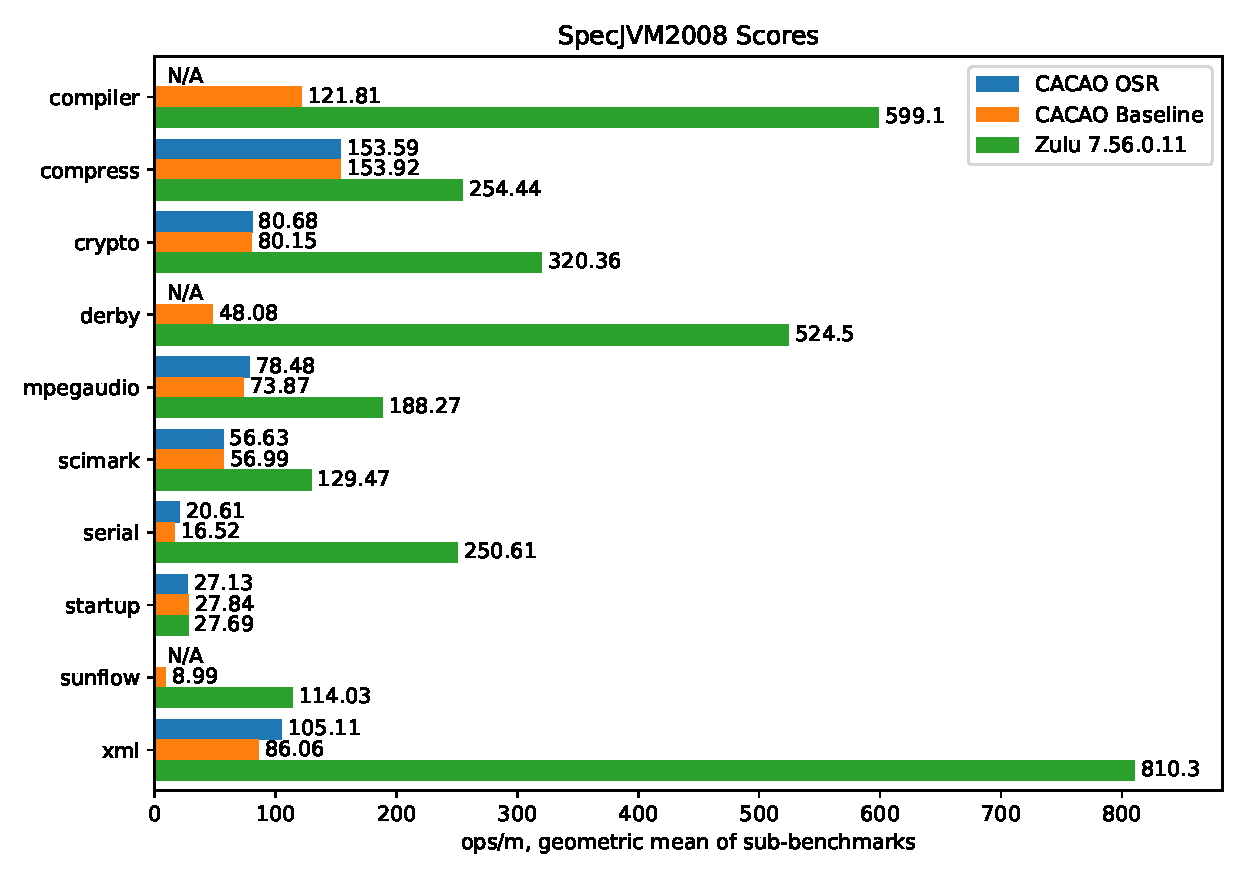
\includegraphics[width=\textwidth]{../evaluation/specjvm/plots/plot3_grouped}
        \caption{Comparison of SpecJVM2008 scores}
        \label{fig:spec-cmp}
    \end{figure}


    Both previously failing compiler2 tests were fixed (Fact, Permut).
    The new JUnit tests helped to detect and fix bugs during development.
    The entire CACAO test suite passes with and without inlining.

    For SpecJVM, all but three benchmarks are passing.
    With compiler2 enabled \lstinline{sunflow} and \lstinline{compiler.compiler} produce invalid results, and \lstinline{derby} doesn't seem to terminate.
    It is difficult to tell whether this is due to OSR or unrelated bugs.

    Figure\ref{fig:spec-cmp} shows the comparison between CACAO with and without OSR,
    and the Azul Zulu JDK 7.
    The impact of OSR can be seen in Figure\ref{fig:spec-relative}.
    The \lstinline{serial} and \lstinline{xml} benchmarks saw the largest improvement of $+24.76\%$ and $+22.14\%$ ops/m respectively,
    while the startup performance got slightly worse.

    \begin{figure}
        \centering
        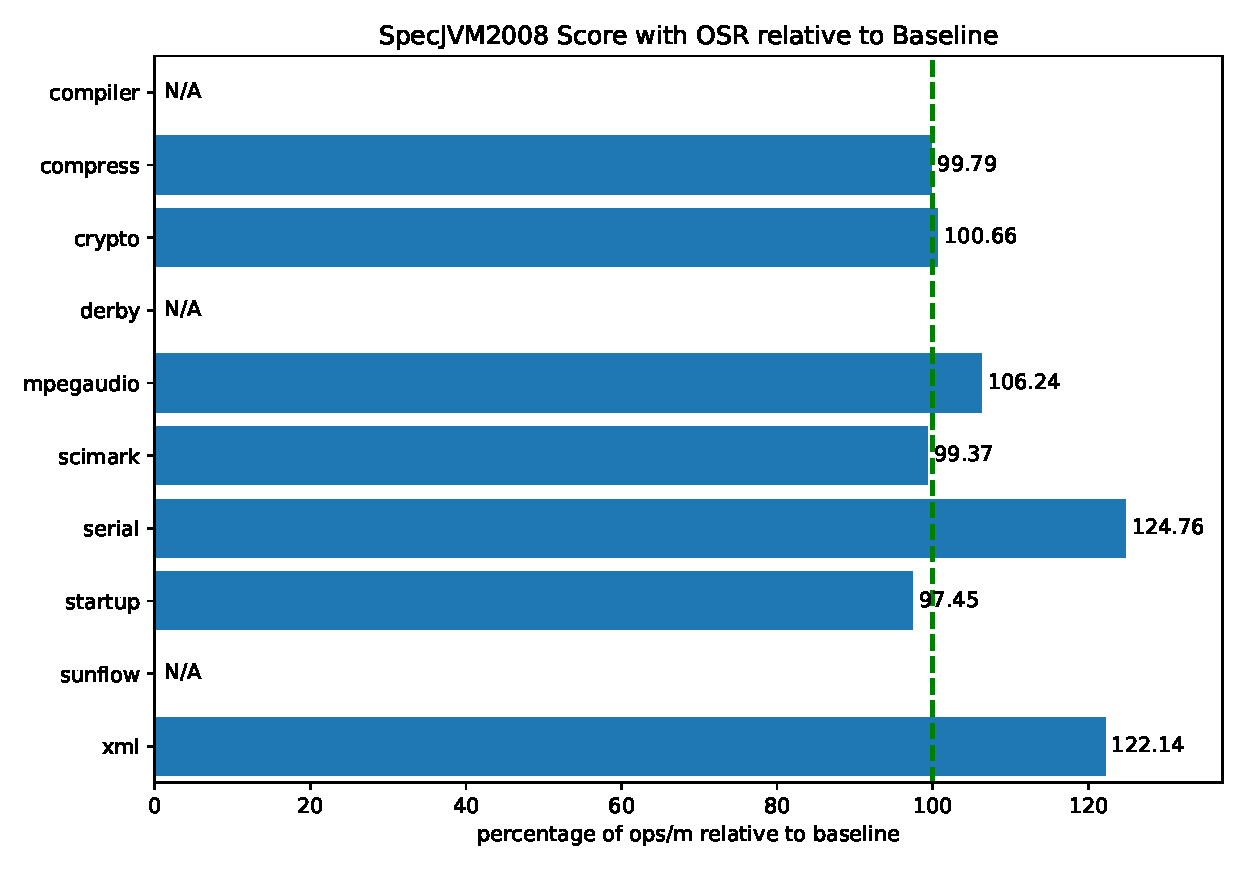
\includegraphics[width=\textwidth]{../evaluation/specjvm/plots/plot_normalized_grouped}
        \caption{Impact of OSR on SpecJVM2008 scores}
        \label{fig:spec-relative}
    \end{figure}

    According to the collected statistics,
    there were 3122 compiler2 calls in total,
    out of which 3032 were successful.
    In 93 cases, the baseline compiler was used,
    but this also includes code for deoptimizations.
    6686 methods didn't get countdown traps
    because they were skipped due to the heuristic.
    The numbers might not be entirely accurate
    because the counters don't use atomic increments.


    \begin{table}
        \centering
        \begin{tabular}{rrl}
            \toprule
            \textbf{At method entry} & \textbf{From within method} & \textbf{Target}        \\
            \midrule
            80                       & 10                          & to baseline, uncached  \\
            470                      & 9                           & to baseline, cached    \\
            \midrule
            2954                     & 78                          & to compiler2, uncached \\
            8071                     & 0                           & to compiler2, cached   \\
            \midrule
            11575                    & 97                          & total                  \\
            \bottomrule
        \end{tabular}
        \caption{Number of on-stack replacements}
        \label{tab:osr-counts}
    \end{table}

    Table\ref{tab:osr-counts} shows where and to which version of the code optimizations happened.
    Surprisingly, the vast majority of them happens at method entry.
    This is likely because the heuristic often rejects more complex methods.

    There were a total of 185 deoptimizations.
    83 were uncached (2.7\% of 3032 optimized methods)
    and in 102 cases the target was already cached.


    \section{Conclusion}

    A basic version of OSR was implemented and tested.
    This uncovered a number of unrelated issues with the new compiler, most of them were fixed.
    Inlining was simplified and works in simple cases,
    but it remains disabled by default
    because larger programs like SpecJVM still trigger assertions and crashes.
    Overall, OSR results in performance improvements for benchmarks.


    \chapter{Future work}


    \section{OSR Improvements}

    Development has been focused only on \texttt{x86\_64}.
    Although \texttt{aarch64} has been taken into account for cases
    such as the location of stack slots,
    it looks like the code for callee-saved registers
    hasn't been compiling since before the start of this work.

    There might also be some edge cases that aren't covered by the current implementation,
    for example, with rare values such as \lstinline{returnAddress}.
    Also, the allocation info of replacement points at call sites is currently never used
    and could be omitted.

    When compiler2 specializes a method to a replacement point,
    it currently reads all values from the stack
    and then does an unconditional branch to the correct basic block.
    It would be better to also have a conditional branch that isn't taken,
    to the original entrypoint,
    to keep that code alive.
    That would then allow constant propagation to replace phi nodes where
    the only different non-constant value is coming from the unconditional branch.

    When lowering source states, the operands could be deduplicated.
    If multiple variables share the same value, it is slightly inefficient
    to require both of them as separate operands.

    There has also been almost no work done on performance.
    Once compiler2 supports compiling most methods,
    multiple variations of OSR could be tried to
    determine which one works best in practice.


    \section{Compiler2 Improvements}

    Compiler2 still has many unsupported instructions.
    Table- and lookupswitch were disabled.
    There are also problems with integer division and modulo
    because they get dead code eliminated and reordered
    even if they could potentially throw an exception.

    Dead code caused quite a few problems during development.
    Since the new solution for scheduling basic blocks completely
    ignores unreachable ones, it should now be easy to add
    constant evaluation of branches.

    Inlining still doesn't work reliably for SpecJVM.
    Also, the budget calculation for the knapsack heuristic might be incorrect,
    and the implementation for guarded inlining is incomplete.


    \section{Breakpoints and Garbage Collection}

    CACAO doesn't support debugging Java code right now,
    but breakpoints would be conceptually very similar to replacement points.
    If a breakpoint was placed into optimized code,
    there would have to be a way to force it to return to the unoptimized variant.

    For garbage collection,
    CACAO currently uses Boehm GC by default.
    There is also an old implementation of a precise garbage collector, but it doesn't work anymore.
    Precise garbage collectors have somewhat similar requirements to OSR.
    They usually require GC safe points where execution can be paused
    and where every reference on the stack can be recovered.
    In the past, this was implemented with replacement points.
    With compiler2, these two concepts would be slightly different, though.
    A replacement point forces a certain set of values to be live,
    while a GC safe point just needs to know about references to heap allocations.
    Also, if optimizations such as scalar replacement were implemented,
    then replacement points could require additional code
    that allocates an object right before deoptimizing.

    \appendix


    \chapter{Detailed SpecJVM results}


    \section{Individual Scores}

    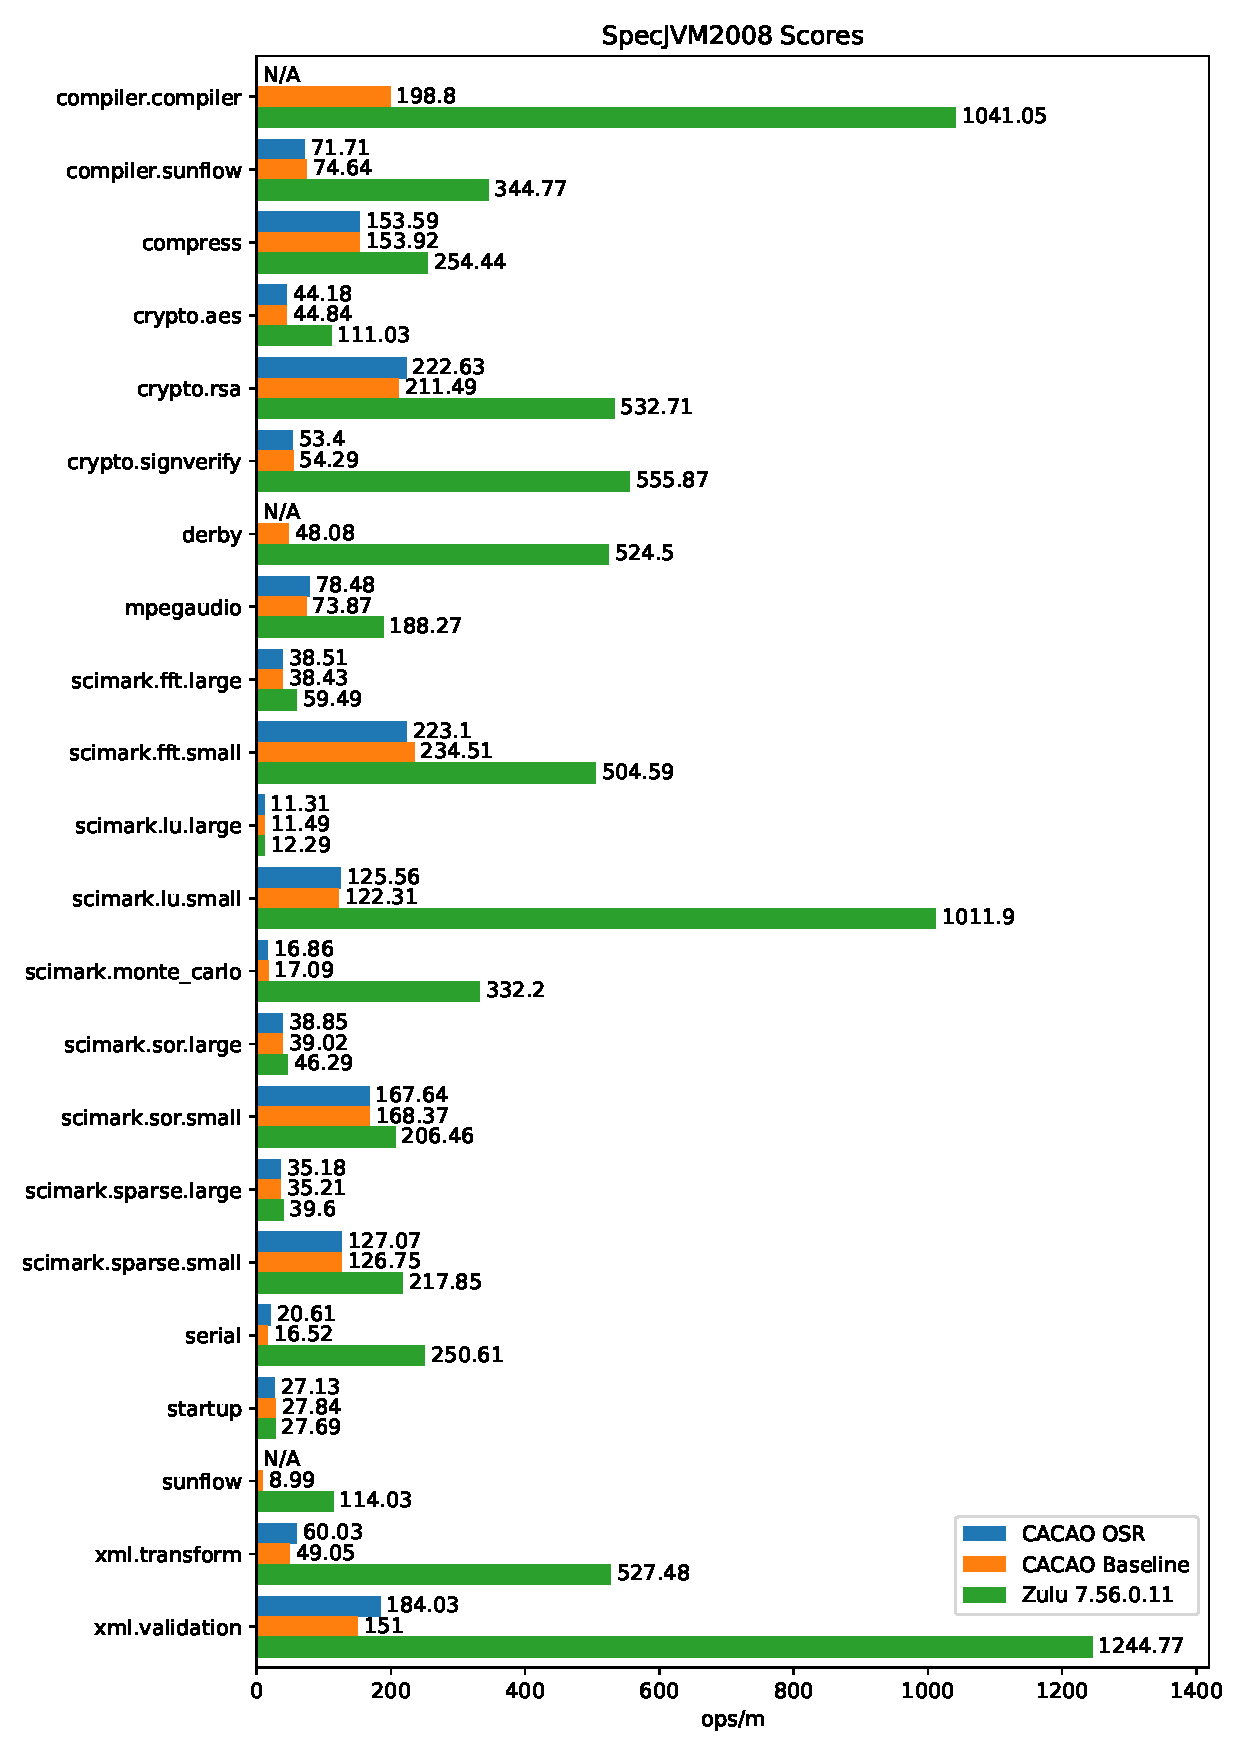
\includegraphics[width=\textwidth]{../evaluation/specjvm/plots/plot3}


    \section{Normalized Comparison}

    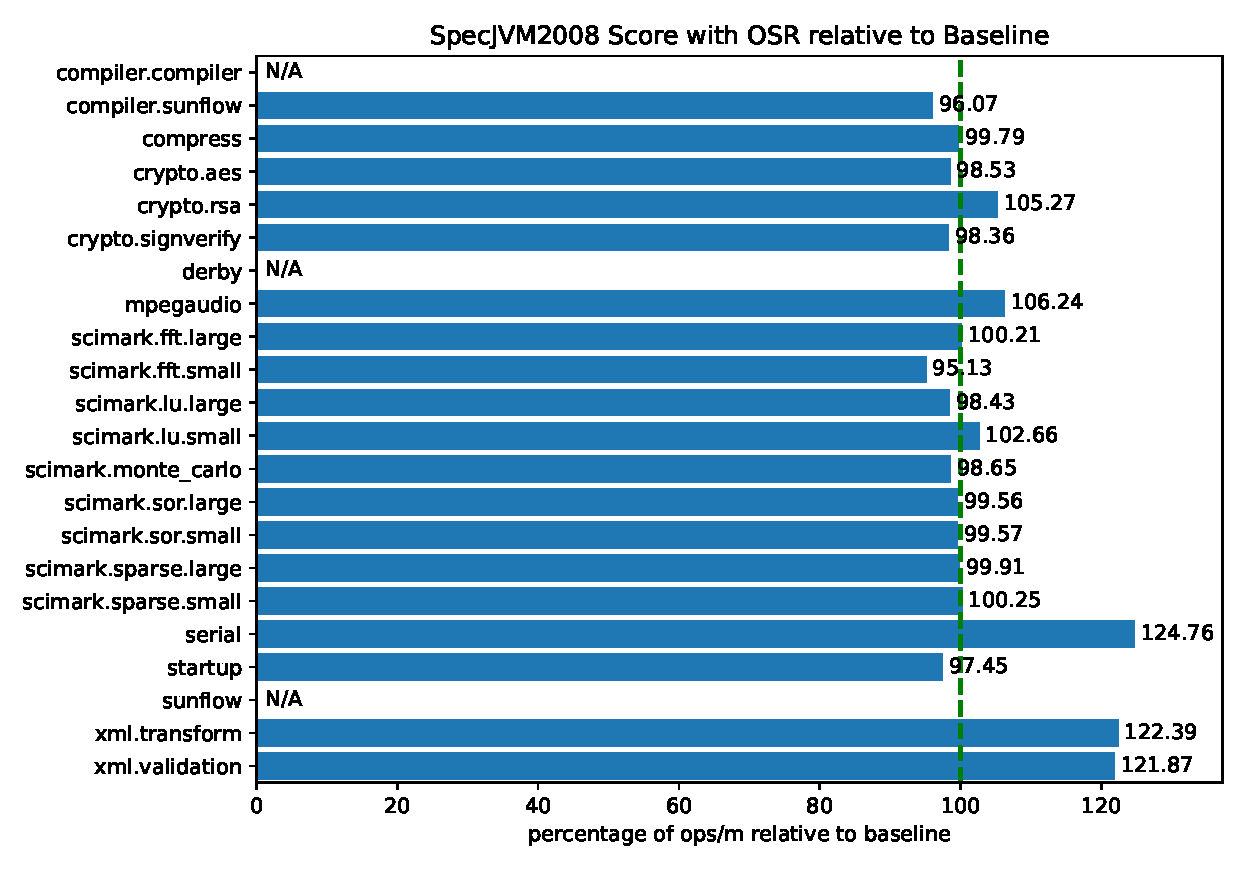
\includegraphics[width=\textwidth]{../evaluation/specjvm/plots/plot_normalized}


    \backmatter

% Use an optional list of figures.
%    \listoffigures % Starred version, i.e., \listoffigures*, removes the toc entry.

% Use an optional list of tables.
%    \cleardoublepage % Start list of tables on the next empty right hand page.
%    \listoftables % Starred version, i.e., \listoftables*, removes the toc entry.

% Use an optional list of alogrithms.
%    \listofalgorithms
%    \addcontentsline{toc}{chapter}{List of Algorithms}

% Add an index.
    \printindex

% Add a glossary.
%    \printglossaries

% Add a bibliography.
%\bibliographystyle{alpha}
    \bibliographystyle{unsrturl}
    \bibliography{main}

\end{document}
